% !TeX program = xelatex
% OrchestraBench -- Agent Evaluation Science (AES) Fall 2026, Short Paper track.
% Compile: latexmk -xelatex main.tex   (pdfLaTeX is not supported by aes.sty)
\documentclass[11pt,a4paper]{article}
\usepackage{aes}

\usepackage{amsmath,tabularx}
\usepackage{tikz}
\usetikzlibrary{arrows.meta,decorations.pathreplacing}
\graphicspath{{figures/}}

\title[OrchestraBench]{OrchestraBench: Evaluating Multi-Agent Orchestration
Failure Modes, Recovery, and Decomposition Quality}

\aesauthor[affil={1}]{Yidian Chen}
\aesauthor[affil={1}]{Yingzi Gu}
\aesauthor[affil={1}]{Natan Vidra}
\aesauthor[affil={1}]{Spurthi Setty}
\aesauthor[affil={1}]{Sharon Zheng}
\aesaffiliation{1}{Anote}

% TODO(authors): add corresponding-author email(s), or leave omitted.
% \aesemails{\aesemail{name@anote.ai}}

\aeskeywords{Agent evaluation; Multi-agent orchestration; Failure injection;
Error propagation; Construct validity}

\begin{document}
\maketitle

\begin{abstract}
Benchmarks for multi-agent orchestration typically report whether a pipeline
succeeded, not why it failed, where an error began, or how far it spread. We
present OrchestraBench, a seed-reproducible failure-injection harness that
treats failure handling as the unit of evaluation, with per-mode recovery and
\emph{cascade radius} (downstream stages corrupted by one injected fault) as
primary metrics. We report four controlled probes. (1)~On a 26-case routing
diagnostic, a keyword/flag router scores 0\% on 10 adversarial cases whose
surface flags are missing or misleading, while a description-reading TF-IDF
router and an LLM router both score 100\%. (2)~Injecting five MAST failure modes
into a verifiable arithmetic chain run by a Claude agent ($n{=}30$ per mode)
yields three tiers: tool faults are recovered (1.00), ambiguous delegation is
partially recovered (0.30), and three latent modes are never recovered (0/30
each; exact 95\% upper bound 0.12).
The ordering is preserved when the same computation is framed as a loan-approval
workflow and across three Claude models, while absolute rates shift. Retry does
not change final success for any mode and increases median time-to-detection
by about 50\%. (3)~A latent fault corrupts about 93\% of downstream stages at
every depth from 3 to 7, so absolute cascade radius grows from 0.93 to 4.67
while the propagation fraction stays flat. (4)~An apparent containment gain from
an LLM repair policy largely disappears when its trusted upstream value is
removed (0.67 to 0.08). The harness is the primary contribution; the probes run
one agent on a controlled chain within a single model family and are not
estimates of production multi-agent reliability.
\end{abstract}

\section{Introduction}
\label{sec:intro}
When a multi-agent pipeline returns a wrong answer, the failure is often
silent: a misrouted or corrupted step still produces plausible output. Widely
used agent benchmarks \citep{agentbench,swebench,odysseybench} score final task
success and cannot say which orchestration decision failed, how far the error
propagated, or whether a recovery policy helped. Failure taxonomies
\citep{mast} and attribution benchmarks \citep{traceelephant,attribution}
\emph{observe} failures post hoc. Intervention studies inject faulty agents
into multi-agent structures and measure performance loss \citep{huang2025resilience},
analyze how errors propagate across communication topologies
\citep{shen2025propagation}, or score reliability under a fault taxonomy
\citep{masfire}. OrchestraBench is complementary: it fixes the injection stage
and measures stage-resolved propagation, time-to-detection, and the effect of
routing, retry, and repair policies on a construct with exact ground truth.

\textbf{Evaluation target.} We ask a narrower question: \emph{if a known fault is injected at a
known stage, can we measure whether it is recovered, how far it propagates, and
whether the routing or retry policy changes either?} OrchestraBench answers this
with controlled, seeded injection on a construct with exact-match ground truth.
The harness is the primary contribution; the experiments demonstrate what
it measures:
\begin{itemize}
  \item A seed-reproducible harness for injecting MAST failure modes into staged
  pipelines, with formally defined recovery, cascade-radius, and
  time-to-detection metrics (\S\ref{sec:bench}).
  \item Evidence that routing failure on adversarial cases is a property of
  \emph{what the router reads}, not task difficulty (\S\ref{sec:exp1}).
  \item A three-tier recovery structure that is stable in ordering across
  framing and model, with retry providing no recovery for non-tool faults
  (\S\ref{sec:exp2}), and a depth-resolved cascade measurement whose
  normalized form separates propagation fraction from chain length
  (\S\ref{sec:exp3}).
  \item An ablation showing how a trusted-state signal can masquerade as
  autonomous detection in containment evaluations (\S\ref{sec:probe}).
\end{itemize}
An earlier version of this work is available as a preprint
\citep{chen2026orchestrabench}; this short paper condenses it and tightens its
claims for an evaluation-methods audience. Code, data, and analysis scripts
are public.\footnote{\url{https://github.com/anote-ai/research-orchestratebench};
dataset: \url{https://huggingface.co/datasets/anote-ai/Orchestratebench}.}

\section{The OrchestraBench Harness}
\label{sec:bench}

\textbf{Construct.} For Experiments~2--4 the pipeline is a \emph{verifiable
arithmetic dependency chain}: a sequence of $d$ stages in which stage $k$
consumes the value produced by stage $k{-}1$. A single agent executes each stage
under a stage-specific prompt. The construct is chosen for exact-match ground
truth at every stage, so no subjective grading is required. A domain-framed
variant re-expresses the identical computation as a four-role loan-approval
workflow (intake, risk, compliance, approval).

\textbf{Failure injection.} A seeded \texttt{FailureInjector} applies one of five
MAST modes \citep{mast} at the prompt level at stage index 1 (the second stage):
\emph{tool-invocation error}, \emph{ambiguous delegation}, \emph{context
pollution}, \emph{conflicting sub-agent outputs}, and \emph{premature action}.
We call the four non-tool modes \emph{latent}, because the fault corrupts state
rather than raising a visible error. Every scenario is regenerable from its seed.

\textbf{Metrics.} For run $i$ with depth $d_i$ and injection at stage $j$, let
$c_{ik}\in\{0,1\}$ indicate that the output of stage $k$ differs from ground
truth. We define
\begin{equation}
  \mathrm{CR}_i=\sum_{k=j+1}^{d_i-1} c_{ik},
  \qquad
  \mathrm{Rec}_m=\frac{1}{|R_m|}\sum_{i\in R_m} s_i,
  \label{eq:metrics}
\end{equation}
where $\mathrm{CR}_i$ is the cascade radius (corrupted stages strictly
downstream of the injection, maximum $d_i{-}2$ here), $R_m$ is the set of runs
injected with mode $m$, and $s_i$ indicates exact-match final-task success.
Because the maximum of $\mathrm{CR}_i$ grows with depth, we also report the
normalized radius $\widetilde{\mathrm{CR}}_i=\mathrm{CR}_i/(d_i{-}j{-}1)$, the
fraction of downstream stages corrupted.
Time-to-detection is wall-clock time until the policy flags the fault or the
run ends. The harness also logs routing accuracy, latency, cost, and
decomposition fidelity (Appendix~\ref{app:exp4}).

\textbf{Policies.} \emph{Fixed} (always one route), \emph{Heuristic}
(keyword and complexity flags), \emph{Retry} (heuristic plus automatic retry),
\emph{LLM-router} (four-way route selection, Exp~1), \emph{LLM-repair} (an LLM
pass at the injected stage that may correct the stage, \S\ref{sec:probe}), and
\emph{Oracle} (gold route or gold repair; a ceiling). Figure~\ref{fig:protocol}
shows where injection and each metric enter a run.

\begin{figure}[htbp]
  \centering
  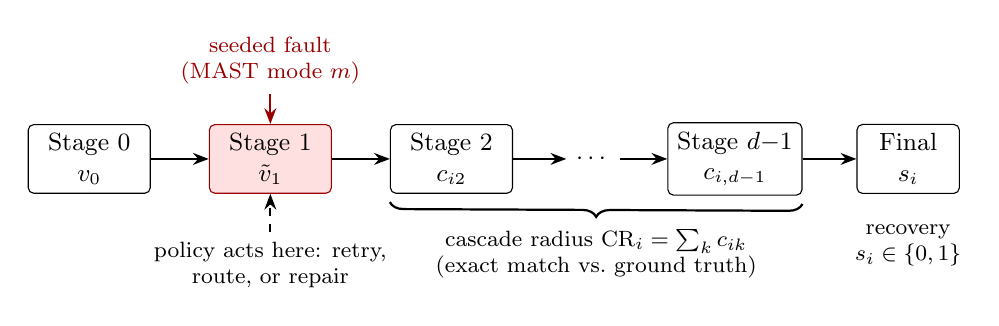
\begin{tikzpicture}[
      st/.style={draw, rounded corners=2pt, minimum width=1.55cm, minimum height=0.8cm, font=\small, align=center},
      ar/.style={-{Stealth[length=2mm]}, thick},
      lab/.style={font=\footnotesize, align=center}]
    \node[st] (s0) at (0,0) {Stage 0\\$v_0$};
    \node[st, fill=red!12, draw=red!60!black] (s1) at (2.3,0) {Stage 1\\$\tilde v_1$};
    \node[st] (s2) at (4.6,0) {Stage 2\\$c_{i2}$};
    \node[font=\small] (dots) at (6.4,0) {$\cdots$};
    \node[st] (sd) at (8.2,0) {Stage $d{-}1$\\$c_{i,d-1}$};
    \node[st, minimum width=1.3cm] (out) at (10.4,0) {Final\\$s_i$};
    \draw[ar] (s0) -- (s1); \draw[ar] (s1) -- (s2); \draw[ar] (s2) -- (dots);
    \draw[ar] (dots) -- (sd); \draw[ar] (sd) -- (out);
    \node[lab, text=red!60!black] (inj) at (2.3,1.25) {seeded fault\\(MAST mode $m$)};
    \draw[ar, red!60!black] (inj) -- (s1);
    \node[lab] (pol) at (2.3,-1.35) {policy acts here: retry,\\route, or repair};
    \draw[ar, dashed] (pol) -- (s1);
    \draw[decorate, decoration={brace, amplitude=5pt, mirror}, thick]
      ([yshift=-3pt]s2.south west) -- ([yshift=-3pt]sd.south east)
      node[midway, below=6pt, lab] {cascade radius $\mathrm{CR}_i=\sum_k c_{ik}$\\(exact match vs.\ ground truth)};
    \node[lab] at (10.4,-1.1) {recovery\\$s_i\in\{0,1\}$};
  \end{tikzpicture}
  \caption{One OrchestraBench run. A seeded fault is injected at stage index~1;
  each downstream stage is checked against ground truth to compute cascade
  radius, the final output gives recovery, and time-to-detection is measured
  until the policy flags the fault or the run ends.}
  \label{fig:protocol}
\end{figure}

\section{Experimental Setup}
\label{sec:setup}
The agent is Claude Sonnet 4.6 (\texttt{claude-sonnet-4-6}) unless noted; the
cross-model check adds \texttt{claude-opus-4-8} and \texttt{claude-haiku-4-5}.
Runs were collected between June 21 and July 3, 2026. Experiment~2 uses depth-4
chains with 10 runs per mode under each of the three baseline policies
($n{=}30$ per mode, $N{=}150$ per framing); Experiment~3 uses depths 3--7
($n{=}120$ latent runs per depth, $N{=}750$). We report 95\% percentile
bootstrap intervals (10{,}000 resamples), Wilson intervals for the Exp~1
proportions, and exact two-sided sign-flip permutation tests for paired
comparisons, because the bootstrap $p$-value is anti-conservative when all
paired differences share a sign. For cells at 0 or 1 we report exact
Clopper--Pearson intervals ($[0, 0.12]$ or $[0.88, 1]$ at $n{=}30$), since the
bootstrap collapses to zero width there. These outcomes are not fixed by the
construct: if a latent corruption persists, the final exact-match check must
fail, but whether the agent detects and repairs it is the behavior being
measured (Opus repairs conflicting outputs in 3 of 30 runs). Total API cost
was about \$4.

\section{Results}
\label{sec:results}

\subsection{Routing depends on what the router reads}
\label{sec:exp1}
The routing diagnostic has 26 author-labelled cases over four routes: 16
\emph{aligned} cases whose surface flags match intent and 10 \emph{adversarial}
cases whose flags are missing or misleading while the description's intent is
unambiguous. The LLM router receives the description and metadata but never the
label, and returns a structured route; results were identical across three
passes (78/78).

\begin{table}[htbp]
  \centering
  \begin{tabularx}{\linewidth}{@{}Xrrr@{}}
    \toprule
    Policy & Overall & Aligned ($n{=}16$) & Adversarial ($n{=}10$) \\
    \midrule
    Fixed (no signal) & 23\% & 25\% & 20\% \\
    Heuristic (keyword/flags) & 62\% & 100\% & 0\% \\
    TF-IDF (reads description) & 92\% & 88\% & 100\% \\
    LLM-router (Sonnet 4.6) & 100\% & 100\% & 100\% \\
    Oracle & 100\% & 100\% & 100\% \\
    \bottomrule
  \end{tabularx}
  \caption{Routing accuracy on the 26-case diagnostic. Wilson 95\% CIs on the
  adversarial cases: Heuristic $[0.00, 0.28]$; TF-IDF and LLM $[0.72, 1.00]$.}
  \label{tab:exp1}
\end{table}

The heuristic falls below the no-signal baseline on adversarial cases (0\% vs.\
20\%), so misleading flags are worse than none (Table~\ref{tab:exp1}). A
TF-IDF router with fixed per-route prototypes and no model recovers every
adversarial case, so the gap is explained by reading the description rather than
by model capability. The diagnostic is constructed as a worst case for flag
matching and saturates for the LLM; it isolates \emph{when} keyword routing
fails, not how routers rank on realistic distributions.

\subsection{Recovery splits into three tiers}
\label{sec:exp2}

\begin{table}[htbp]
  \centering
  \begin{tabularx}{\linewidth}{@{}Xcccc@{}}
    \toprule
    & \multicolumn{2}{c}{Sonnet 4.6} & Opus 4.8 & Haiku 4.5 \\
    \cmidrule(lr){2-3}
    Failure mode & Arithmetic & Loan approval & Arithmetic & Arithmetic \\
    \midrule
    Tool-invocation error & 1.00 & 0.70 [0.53, 0.87] & 1.00 & 1.00 \\
    Ambiguous delegation & 0.30 [0.13, 0.47] & 0.40 [0.23, 0.57] & 0.10 & 0.20 \\
    Context pollution & 0.00 & 0.00 & 0.00 & 0.00 \\
    Conflicting outputs & 0.00 & 0.00 & 0.10 & 0.00 \\
    Premature action & 0.00 & 0.00 & 0.00 & 0.00 \\
    \bottomrule
  \end{tabularx}
  \caption{Final-task success by injected mode ($n{=}30$ per cell). Brackets are
  95\% bootstrap CIs; every 0.00 cell has exact 95\% CI $[0, 0.12]$ and every
  1.00 cell $[0.88, 1]$. Mean cascade radius on the depth-4
  chain is 0.00 for tool faults, 1.40 for ambiguous delegation, and 2.00 (the
  maximum) for the other three modes.}
  \label{tab:exp2}
\end{table}

Table~\ref{tab:exp2} shows three tiers on the arithmetic chain. The agent
recomputes by hand when a tool fails (success 1.00, cascade 0), infers the
intended operation in about a third of ambiguous delegations, and never recovers
from context pollution, conflicting outputs, or premature action. Two checks
bear on whether this reflects agent behavior or only the chain's structure.
First, under the loan-approval framing the ordering holds but rates move: tool
recovery drops to 0.70 and ambiguous delegation rises to 0.40
(Figure~\ref{fig:exp2} in Appendix~\ref{app:figs}). Second, across three Claude
models, tool faults are always recovered and context pollution and premature
action never are; only ambiguous delegation (0.10--0.33) and one Opus cell
(conflicting outputs, 0.10) vary. Because the cross-model cells use $n{=}30$
and a single model family, we read this as consistency of ordering, not model
invariance. The Sonnet cross-model run is also an independent repeat of the main
probe: it reproduces all five cells (ambiguous delegation 0.33 vs.\ 0.30, the
rest identical), a test--retest check on the harness itself.

\textbf{Retry does not repair latent faults.} Final-task success is identical
under Fixed, Heuristic, and Retry for every mode (e.g.\ 0.30 for ambiguous
delegation under all three), while median time-to-detection rises from 4.1--4.3\,s
to 6.2\,s under Retry. Retrying with the corrupted state intact reproduces the
error. For evaluation design, this means a recovery metric that counts retries
as recovery attempts will over-credit retry policies unless it also checks
whether the fault was attributed and the state repaired.

\subsection{Propagation fraction is constant across depth}
\label{sec:exp3}
Injecting one fault at stage index 1 of chains of depth 3--7, raw latent
cascade radius grows from 0.93 [0.88, 0.97] to 1.85, 2.80, 3.63, and 4.67
[4.42, 4.88] (Figure~\ref{fig:exp3}), while tool faults stay at 0. Normalized by
the maximum $d{-}2$, the corrupted fraction is flat: 0.93, 0.93, 0.93, 0.91,
and 0.93. Deeper chains therefore do not make a latent fault more likely to
spread; it corrupts nearly every downstream stage at every depth, and absolute
damage grows only because there are more stages. The three non-recovering modes
sit at the maximum, and ambiguous delegation corrupts a stable 0.63--0.73 of
downstream stages. Reporting only raw cascade radius would suggest increasing
propagation propensity, which these data do not support.

\begin{figure}[htbp]
  \centering
  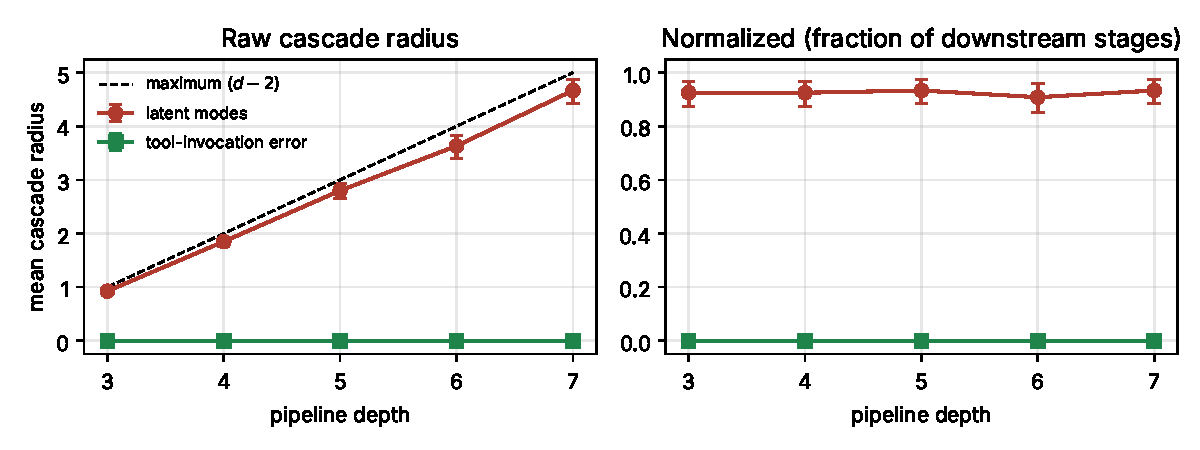
\includegraphics[width=\linewidth]{exp3_cascade_raw_norm.pdf}
  \caption{Cascade radius by pipeline depth (Sonnet 4.6, $N{=}750$; 95\% bootstrap
  CIs). Left: raw radius tracks the maximum $d{-}2$. Right: normalized by that
  maximum, the latent corrupted fraction stays near 0.93 at every depth.}
  \label{fig:exp3}
\end{figure}

\subsection{Trusted state can masquerade as detection}
\label{sec:probe}
We next ask whether a policy can contain latent cascades. The LLM-repair policy
runs an LLM pass at the injected stage that is given the trusted upstream value
and permitted to correct the stage; it is distinct from the Exp~1 LLM-router. Under this setting, latent recovery is 0.83
[0.58, 1.00] versus 0.08 for the baselines and 1.00 for Oracle, and the gap
widens with depth (Appendix~\ref{app:probe}). An ablation removes only the
trusted upstream value (LLM-repair without upstream): in an independent sweep
($N{=}180$), latent recovery falls from 0.67 [0.46, 0.83] to 0.08 [0.00, 0.21],
the baseline level (paired drop 0.58 [0.33, 0.79], exact $p{=}5.2{\times}10^{-4}$,
24 pairs). The apparent containment is mostly the trusted-state signal, not
autonomous detection. We include this result because the same confound can
arise in any containment evaluation that gives the evaluated policy access to
ground-truth or privileged state.

\section{Implications for Evaluation Practice}
\label{sec:discussion}
Four practices follow from these probes. First, report recovery \emph{per
failure mode}: the pooled latent success rate (0.075 on the arithmetic chain)
hides a tool-vs-latent split that is the most stable finding here. Second,
separate retry from repair, and record time-to-detection, since retry changes
cost and latency without changing outcomes for latent faults. Third, ablate
privileged information available to any policy whose containment is being
measured; in our case it accounted for most of the measured gain. Fourth,
report cascade radius normalized by its topology-implied maximum: in our data
the raw radius grows fivefold with depth while the normalized radius does not
change.

\section{Limitations}
\label{sec:limitations}
\begin{itemize}
  \item \textbf{Construct validity.} Experiments~2--4 use one agent on an
  arithmetic chain with prompt-level injection, not independent agents on
  real workflows or multi-agent frameworks.
  The domain re-framing changes the prompts but not the computation; the
  finance, HR, and DevOps suites in the harness have not yet been evaluated.
  \item \textbf{Model coverage.} All results use Claude models; the cross-model
  check covers three Claude tiers at $n{=}30$ per cell. Non-Claude models are
  untested.
  \item \textbf{Missing controls.} We did not run matched no-injection chains,
  so baseline execution errors are not separated from injected-fault effects.
  Injection provenance is known by design; the harness does not yet test
  whether a policy can \emph{infer} which mode and stage failed.
  \item \textbf{Sample size.} The routing diagnostic has 26 author-labelled cases
  with no inter-annotator agreement, and it saturates. The policy probe has about
  12 latent runs per policy, so its interval for the LLM row is wide.
  \item \textbf{Policy semantics.} The LLM-repair policy's access to trusted state is a
  modelling choice; the ablation bounds its effect but a deployable router
  without that access was not evaluated.
\end{itemize}

\section{Conclusion}
\label{sec:conclusion}
OrchestraBench measures orchestration by how failures are handled rather than by
final success. On controlled probes, routing failure tracks what the router
reads, recovery separates tool faults from latent faults in a way that is
stable in ordering across framing and model, retry does not repair latent
faults, and an apparent containment gain is mostly a trusted-state signal. The
main open question is whether the tool-vs-latent split holds on multi-agent
systems running real enterprise workflows.

\begin{aespubliconly}
\aesbackmattersection{Acknowledgments}
We thank the Anote AI Research Fellowship for support.
\end{aespubliconly}

\aesbackmattersection{Ethics Statement}
OrchestraBench evaluates the reliability of automated orchestration and is
intended to surface silent failures before deployment. All workflows are
synthetic and contain no real applicants, employees, customers, or proprietary
records; no human-subjects data is used. The injected modes come from a public
taxonomy \citep{mast}, so the benchmark adds measurement rather than new attack
techniques. A high score should not be read as evidence of production safety,
and held-out seeded scenarios mitigate overfitting to the injected modes.
Generative AI tools were used for limited editing and coding assistance; all
results and citations were checked against the committed code, data, and cited
records.

\bibliography{references}

\appendix

\section{Related Work}
\label{app:related}

\begin{table}[htbp]
  \centering
  \small
  \begin{tabularx}{\linewidth}{@{}p{3.2cm}XX@{}}
    \toprule
    Prior work & What it does & Difference from OrchestraBench \\
    \midrule
    MAST \citep{mast} & Taxonomy of 14 observed MAS failure modes (1{,}600+ traces) &
    We inject MAST modes under seed control and measure recovery and cascade per mode \\
    MAS-FIRE \citep{masfire} & Fault injection and reliability scoring; 15 fault
    types across MetaGPT, Table-Critic, CAMEL & We add depth-resolved cascade
    radius and vary routing and retry policy \\
    Faulty-agent resilience \citep{huang2025resilience} & Injects errors into agent
    messages across real MAS structures; measures task performance loss and
    repair mechanisms & Real MAS, but outcome-level; we measure per-stage
    propagation and time-to-detection on exact ground truth \\
    Topology propagation \citep{shen2025propagation} & Studies error and
    information propagation across communication topologies; proposes
    EIB-Learner & Varies topology; we fix a chain and vary fault mode, depth, and
    policy \\
    TraceElephant \citep{traceelephant}; Who\&When \citep{attribution} & Post-hoc
    failure attribution benchmarks & Observational; we use controlled seeding \\
    Orchestration patterns \citep{orchpattern} & Accuracy--cost comparison of
    architectures on SEC filings & Complementary; we evaluate failure handling \\
    AdaptOrch \citep{adaptorch} & Task-adaptive orchestration method & A method
    OrchestraBench could evaluate \\
    Spark to Fire \citep{sparkfire} & Models error cascades in MAS collaboration &
    We operationalize cascades as a stage-count metric \\
    DevIntent \citep{devintent} & Measures how often generated code that passes
    visible tests violates unstated developer constraints & Same concern that
    surface success overstates reliability; we study orchestration failures rather
    than single-model code generation \\
    \bottomrule
  \end{tabularx}
  \caption{OrchestraBench relative to closely related work.}
  \label{tab:related}
\end{table}

As a motivating data point, \citet{beyondstrongest} report that on GPQA-Diamond
at least one agent was correct in 95.5\% of cases, while orchestration reached
87.4\%, a loss that failure-level evaluation is intended to localize.

\section{Additional Figures}
\label{app:figs}

\begin{figure}[htbp]
  \centering
  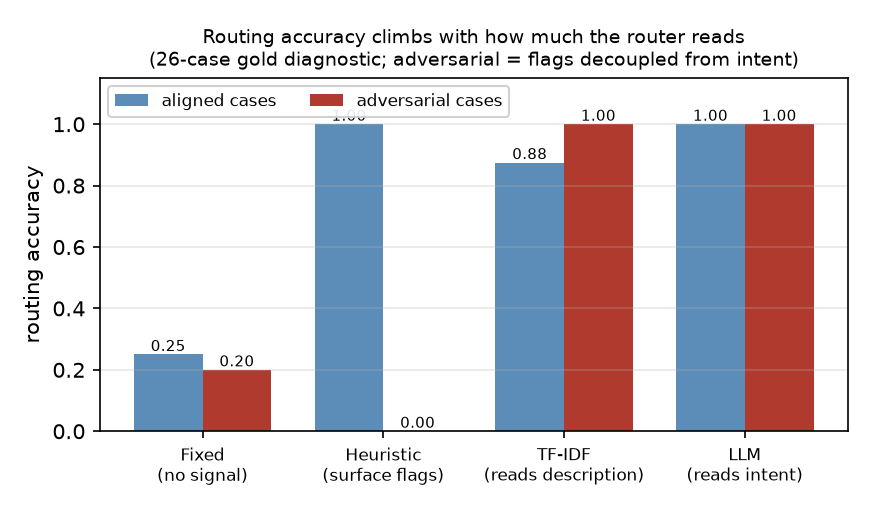
\includegraphics[width=0.8\linewidth]{exp1_routing_ladder.png}
  \caption{Routing accuracy on aligned and adversarial cases for the Exp~1
  diagnostic (data as in Table~\ref{tab:exp1}).}
  \label{fig:exp1}
\end{figure}

\begin{figure}[htbp]
  \centering
  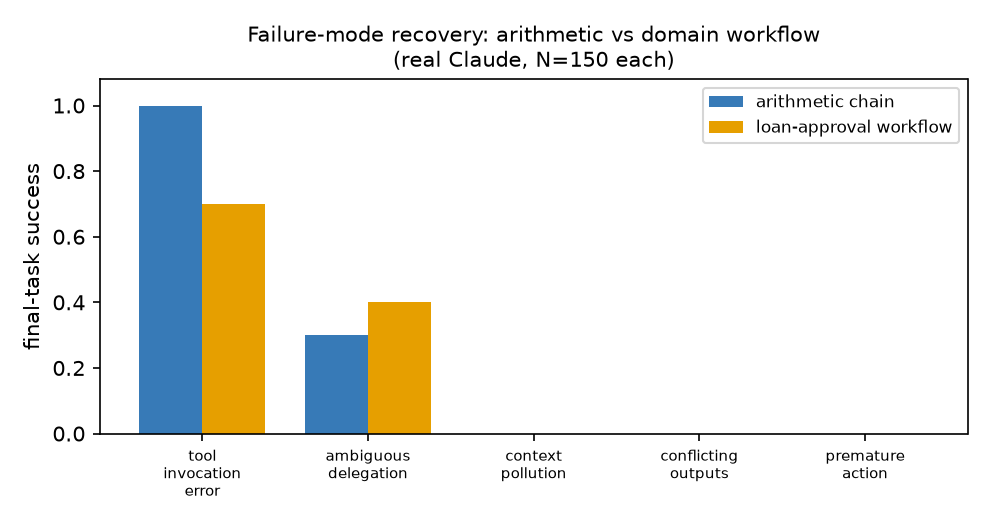
\includegraphics[width=0.8\linewidth]{exp2_arith_vs_domain.png}
  \caption{Final-task success by failure mode, arithmetic chain vs.\ loan-approval
  framing (Sonnet 4.6, $N{=}150$ each).}
  \label{fig:exp2}
\end{figure}

\section{Decomposition Quality (Exploratory)}
\label{app:exp4}
This probe is exploratory: it measures agreement with a canonical decomposition
and does not yet test whether higher fidelity improves localization or recovery.
For composite tasks $(a \mathbin{op} b) \mathbin{op} (c \mathbin{op} d)$ with a
canonical three-step gold decomposition, we compare a \texttt{decompose}
(planner) policy to a \texttt{monolithic} policy ($N{=}40$, 20 shared tasks).
Both reach the correct final answer in every case (1.00). Delegation fidelity
(fraction of gold sub-results exposed) is 1.00 for \texttt{decompose} and 0.37
[0.33, 0.42] for \texttt{monolithic} (paired difference $+0.63$ [0.58, 0.67],
exact $p{=}1.9{\times}10^{-6}$); granularity error is 0 vs.\ 2. Final
correctness alone does not distinguish the policies; the difference is whether
the output exposes sub-results that a planner can delegate, audit, or repair.

\section{Policy-Conditioned Containment}
\label{app:probe}

\begin{table}[htbp]
  \centering
  \begin{tabularx}{\linewidth}{@{}Xcc@{}}
    \toprule
    Policy & Latent recovery & Cascade radius \\
    \midrule
    Fixed / Heuristic / Retry & 0.08 [0.00, 0.25] & 1.83 [1.50, 2.00] \\
    LLM-repair (trusted upstream) & 0.83 [0.58, 1.00] & 0.33 [0.00, 0.83] \\
    Oracle & 1.00 & 0.00 \\
    \bottomrule
  \end{tabularx}
  \caption{Policy-conditioned containment on latent faults, depth-4 chain
  (Sonnet 4.6, $N{=}75$; 95\% bootstrap CIs).}
  \label{tab:policy}
\end{table}

\begin{figure}[htbp]
  \centering
  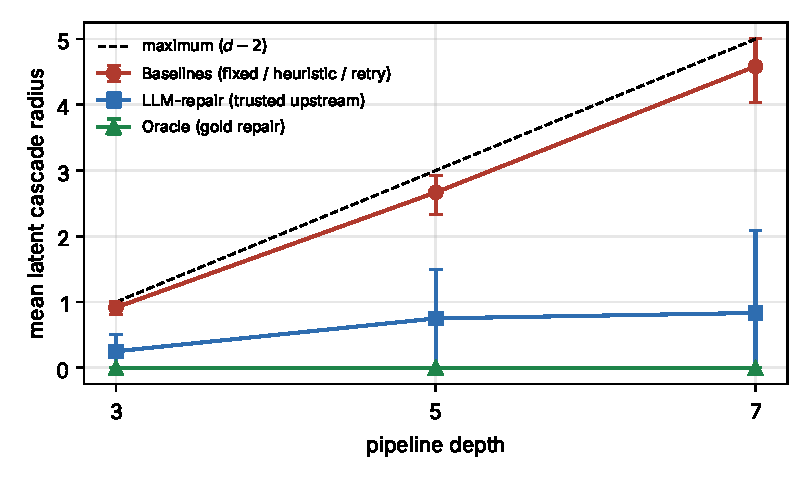
\includegraphics[width=0.75\linewidth]{exp3_policy_cascade.pdf}
  \caption{Latent cascade radius by depth per policy ($N{=}225$; 95\% bootstrap
  CIs; 36 latent runs per depth for the pooled baselines, 12 for LLM-repair and
  Oracle). Baselines track the maximum (0.92, 2.67, 4.58 at depths 3, 5, 7);
  LLM-repair with trusted upstream state stays low (0.25, 0.75, 0.83); Oracle
  is 0.}
  \label{fig:policy}
\end{figure}

\section{Reproducibility}
\label{app:repro}
Scenarios are regenerable from fixed seeds. \texttt{scripts/analyze\_measured.py}
recomputes every Exp~2--4 and policy-probe number in this paper, with bootstrap
intervals and exact permutation tests, offline from the committed CSVs in
\texttt{data/measured/}; we re-ran it on October 20, 2026 and all reported values
matched. The Exp~1 script regenerates Table~\ref{tab:exp1} from the committed
gold set (the LLM row requires an API key). A model-agnostic harness re-runs the
five-mode probe on any model list. Code is Apache-2.0; the test suite (151 tests)
runs offline on Python 3.10--3.12.

\end{document}
